\subsection{Common co-occurring code}

We collect the original GitHub files which contain the similar counterparts, then we extract all co-occurred methods from these GitHub files. For each co-occurring method in each GitHub file, we cluster its similar counterparts from other files. We keep only the clusters with size of at least two and return the remaining clusters in descending order of size.

For 11,110 out of 21K SO queries, we can retrieve common, co-occurring code fragments from GitHub. That is, using our SO query code base and GitHub search code corpus, we can find common co-occurring code for 52.4\% of the queries. The SO queries have a median of 24 common co-occurring methods in GitHub and a mean of 74. The retrieved methods have a median of 12 average lines of code, and a mean of 14 average lines of code. The distribution of number of retrieved methods and distribution of average lines of code are shown in Figure \ref{fig:num-related} and \ref{fig:avg-loc} respectively.
From the figures we can see that a SO query is most likely to have less than ten common co-occurring code fragments, and most of the SO queries have less than 50 common co-occurring methods in GitHub. Most retrieved methods for a query will have five to thirty average lines of code.

\begin{figure}
	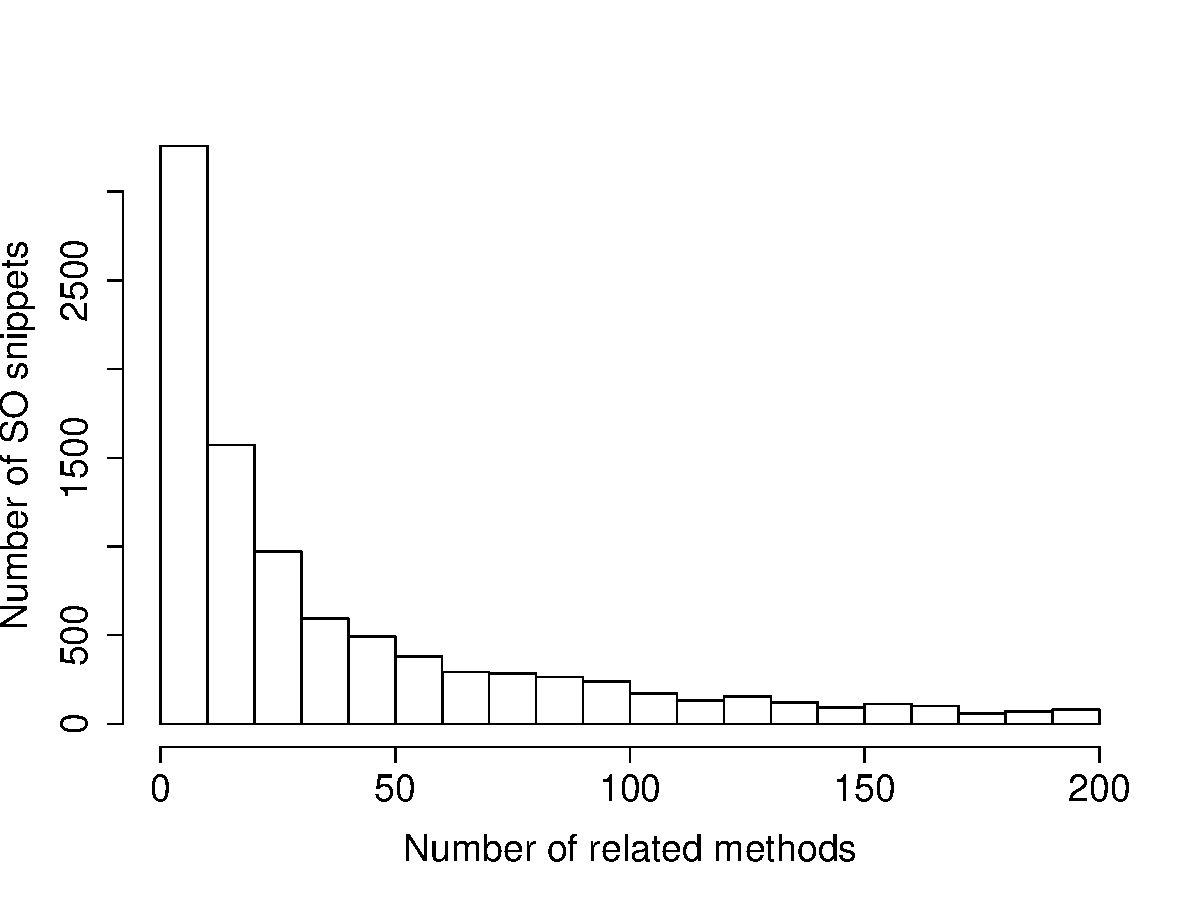
\includegraphics[scale=0.4]{figures/dist-related.pdf}
	\caption{Distribution of number of common co-occurring methods}
	\label{fig:num-related}
\end{figure}

\begin{figure}
	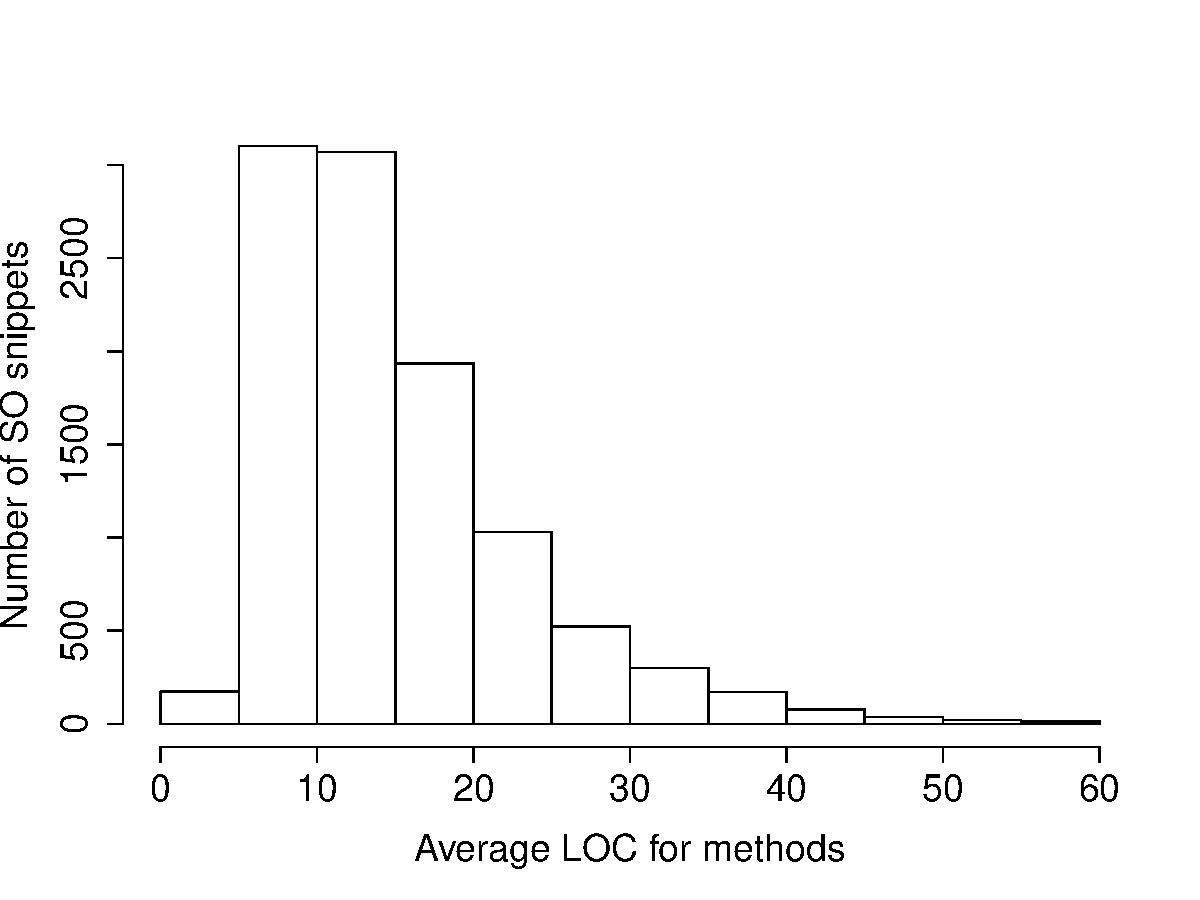
\includegraphics[scale=0.4]{figures/dist-loc.pdf}
	\caption{Distribution of average LOC of common co-occurring methods}
	\label{fig:avg-loc}
\end{figure}

